\documentclass[12pt,a4paper]{article}
\usepackage[utf8]{inputenc}
\usepackage[francais]{babel}
\usepackage[T1]{fontenc}
\usepackage{lmodern,amsmath}
\usepackage[bmargin=1.5cm]{geometry}
\usepackage[sujet,correction]{pas-correction}
	\titlesubject{Exercice sur Scratch}
	\titlecorrection{Correction de l'exercice}
\begin{document}
Ana exécute le programme suivant :

\begin{center}
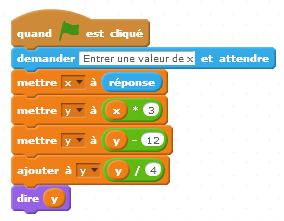
\includegraphics{scratch01.png}
\end{center}

\begin{enumerate}
	\item
	\begin{enumerate}
		\item  Vérifier que si on entre la valeur 8 au départ, on obtient un résultat égal à 3.
		\begin{correction}
		Si on entre 8 au départ, alors $x=8$.
		
		Ensuite, $y=8\times3=24$.
		
		Après, $y=24-12=12$.
		
		Enfin, y=$12 \div 4=3$.
		
		\medskip
		
		On obtient donc bien 3.
		\end{correction}
		\item Quel est le résultat obtenu si on entre la valeur $-1$ au départ ?
		\begin{correction}
		Si on entre $-1$ au départ, alors $x=-1$.
		
		Ensuite, $y=-1\times3=-3$.
		
		Après, $y=-3-12=-15$.
		
		Enfin, y=$-15 \div 4=3,75$.
		
		\medskip
		
		On obtient donc 3,75.
		\end{correction}
	\end{enumerate}
	\newpageforcorrection
	\item Simon prétend que la fonction $f$ définie par :
\[
f(x)=\frac34x-3
\]
donne directement le résultat.

Que penser de cette affirmation ?
\begin{correction}
Si on regarde bien la valeur prise par $y$, on a :
\[
y=\dfrac{3x-12}{4}=\dfrac{3}{4}x-\dfrac{12}{4}=\dfrac{3}{4}x-3=f(x).
\]
Simon a donc raison.
\end{correction}
	\item Quel nombre faut-il entrer au départ pour obtenir un résultat égal à 20 ?
	\begin{correction}
	On souhaite trouver $x$ pour que $f(x)=20$.
	\begin{align*}
	f(x)=20 & \iff \dfrac{3}{4}x-3=20\\
	&\iff \dfrac{3}{4}x=23\\
	&\iff x=23\times\dfrac{4}{3}\\
	&\iff x=\dfrac{92}{3}
	\end{align*}
	Il faudra donc rentrer au départ la valeur $\dfrac{92}{3}$.
	\end{correction}
\end{enumerate}
\end{document}